\paragraph{\texttt{FormInput}}  \mbox{}\\


This component renders a labeled input field with validation feedback. It is designed for use in forms and supports binding with \texttt{v-model} via the \texttt{modelValue} prop. The label and input are semantically linked using the \texttt{id} attribute. Error messages can be displayed below the input when validation fails.

\begin{center}
    \begin{tabularx}{\textwidth}{|X|X|X|X|}
        \hline
        \textbf{Prop} & Type & Required & Description \\
        \hline
        \texttt{id} & \texttt{string} & yes & Unique identifier for the input, used to associate the label \\
        \hline
        \texttt{modelValue} & \texttt{string} & no & The current value of the input (used with \texttt{v-model}) \\
        \hline
        \texttt{label} & \texttt{string} & yes & The text displayed in the label above the input \\
        \hline
        \texttt{type} & \texttt{string} & no & The HTML input type (e.g., \texttt{text}, \texttt{email}, \texttt{password}) \\
        \hline
        \texttt{placeholder} & \texttt{string} & no & Placeholder text inside the input field \\
        \hline
        \texttt{required} & \texttt{boolean} & no & Whether the input is required \\
        \hline
        \texttt{error} & \texttt{string} & no & Displays a red error message below the input if set \\
        \hline
    \end{tabularx}
\end{center}

\paragraph{Emits}
\begin{itemize}
    \item \texttt{update:modelValue} – Emitted on every input change to update the bound model
\end{itemize}



\begin{figure}[H]
    \centering
    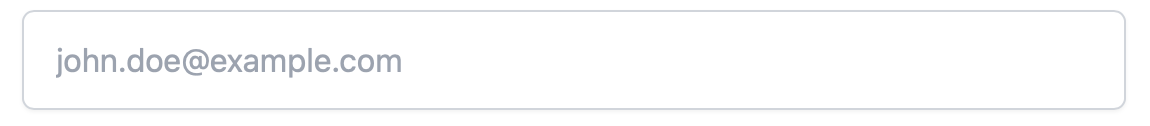
\includegraphics[width=0.7\textwidth]{asset/formInput}
    \caption{\texttt{FormInput}}
\end{figure}
